\cite{FP}
% ==================================================
%	Aufbau
% ==================================================

\section{Aufbau}
\begin{figure}
\centering
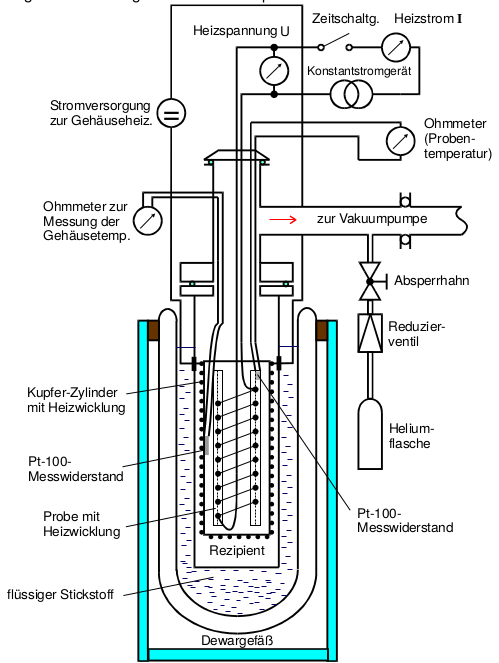
\includegraphics[scale=0.5]{bilder/setup.png}
\caption{Schematische Abbildung des Versuchsaufbaus. \cite{FP}}
\label{fig:aufbau}
\end{figure}
Der Versuchsaufbau ist in Abbildung~\ref{fig:aufbau} zu sehen. 
Die Kupfer-Probe  befindet sich von einem Kupfer-Zylinder umgeben 
in einem Rezipienten. Sowohl Probe als auch Zylinder sind mit jeweils einer 
Heizwicklung und einem Pt-100-Messwiderstand versehen, um Sie getrennt 
voneinander heizen und die Temperatur bestimmen zu können.
Der Rezipient befindet sich in einem Dewargefäß. Er kann mit Hilfe einer 
Vakuumpumpe evakuiert werden. Außerdem kann er über ein Ventil mit 
Heliumgas befüllt werden.

Für die Temperaturmessung mit Hilfe des Messwiderstandes gilt die Beziehung
\begin{equation}
T = 0.00135 \left(\frac{R}{\si{\ohm}}\right)^2 \si{\celsius}+ 2.296 
\left(\frac{R}{\si{\ohm}} \right) \si{\celsius}-243.02 \si{\celsius}
\label{eq:T_berechnung}
\end{equation}
zwischen dem gemessenen Widerstandswert $R$ und der Temperatur $T$.
